\section{Implementation}
\label{sec:implementation_full}
The current cutting voxel projector implementation is part of a larger framework for CBCT reconstruction available at \url{https://github.com/kulvait/kct_cbct} developped by the first author. It is a set of tools written in C++ and OpenCL optimized to run on GPU architectures with fast local memory. The software is released under the open source license GNU GPL3.

\subsection{Calculating voxel cuts}
\label{sec:cuts}
To simplify the calculation of the voxel cuts, we assume a geometric arrangement where the $\chi_2$ axis of the detector is parallel to the $x_3$ axis of world coordinates and by convention their directions are opposite, see Figure \ref{fig:carmconventionalsetup}. This arrangement is used in most current CT trajectories, including the circular trajectory, and is also assumed by footprint projectors, see \cite{Long2010}.

\begin{figure}
    \centering
    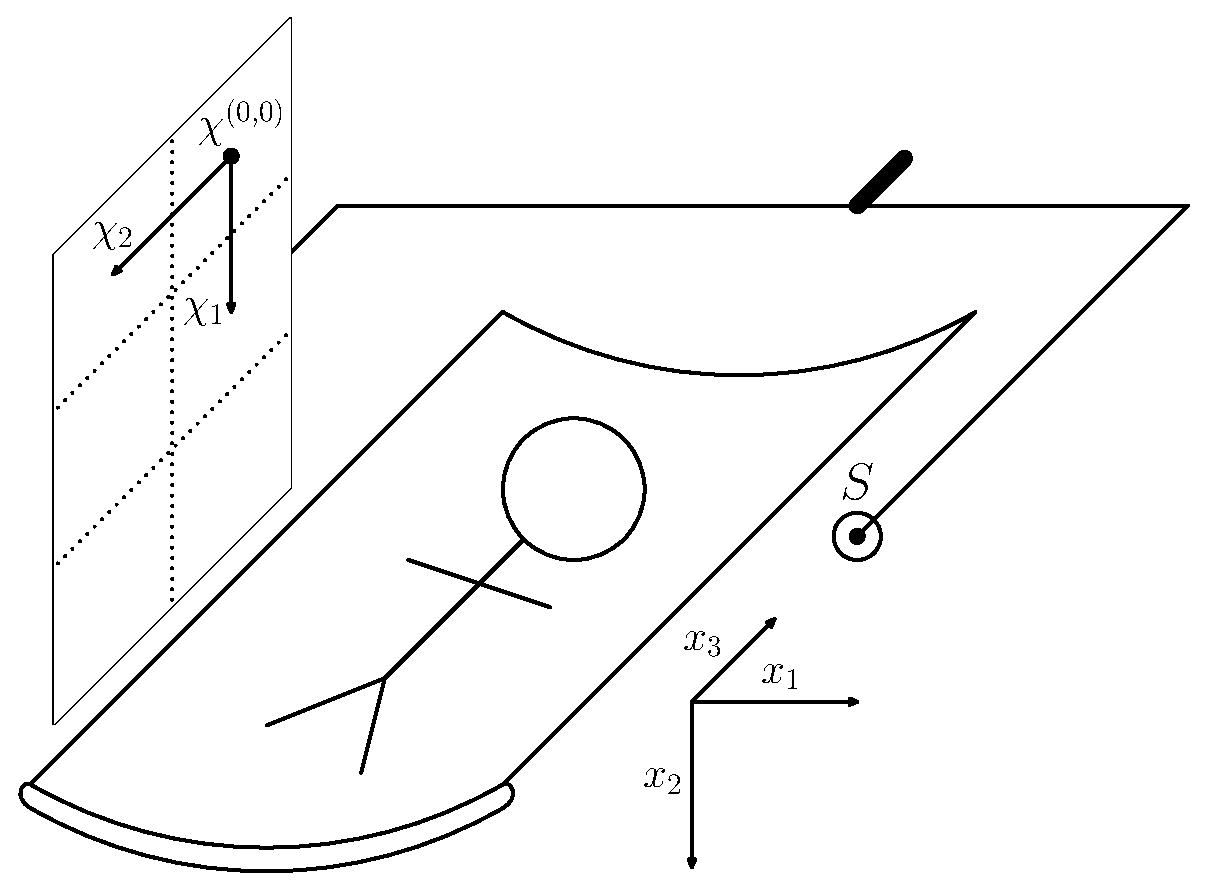
\includegraphics[width=0.45\textwidth]{CTGeometryConstraintsV05.eps}
    \caption{Geometric convention and simplification for the classical cone beam CT arrangement. The axis of rotation is parallel to the $x_3$ axis of world coordinates. In addition, the $x_3$ axis is parallel to the $\chi_2$ axis of the detector, but they have opposite orientations. The origin of the detector is placed in the center of the corner pixel. This arrangement is also assumed in the software.}
    \label{fig:carmconventionalsetup}
\end{figure}

Then, for any two points $x^I = (x_1,x_2,x_3)$ and $x^{II}= (x_1,x_2,x_3')$, which differ only in the value of the third world coordinate it holds that 
\begin{equation}
    \chi_1(x^I) = \chi_1(x^{II}). \label{eq:columnprojectionidentity}
\end{equation}
Therefore, the projection onto the $\chi_1$ is independent of the value of $x_3$. That means that the profiles of the cuts through a given voxel in the $x_1 x_2$ plane will be the same for all $x_3$ coordinates of given voxel and moreover they will be the same for all the voxels with the same fixed $i$ and $j$ indices $V^{i,j,.}$. 

Based on this observation, we first find for each voxel $V^{i,j,k}$ and coordinate $n$ on the detector the polygons $H^{i,j}_n$ into which the base of the voxel parallel with the $x_1x_2$ plane is cut by rays directed to pixels in the $n$-th column of the projector. Our current implementation first finds the corners of the voxel base with the smallest and largest projections $\chi_1^{min}$ and $\chi_1^{max}$. From this we determine the range of allowable integer values $n$ of the column indices of the pixels on the detector on which the voxel is projected. Next, for a given index $n$ we find a polygon $H-^{i, j}_n$ given by the cut of the voxel basis corresponding to projections in the range $\chi_1 \in [\chi_1^{min}, n-0.5]$ and a polygon $H+^{i, j}_n$ corresponding to projections in the range $\chi_1 \in [\chi_1^{min}, n+0.5]$. Finally, we find the polygon $H^{i, j}_n$ as the difference of the sets $H+^{i, j}_n \setminus H-^{i, j}_n$. We compute the area $A_{n}^{i,j}$ and the position of the center of the mass of these polygons being e.g. $\vec{CM}_n^{i,j} = (x_1^{CM},x_2^{CM})$. 

Then, for a given voxel, we reduce the cut in the $x_1 x_2$ plane to its center of mass and find the positions of the $x_3$ breakpoints, which correspond to the projections onto the pixel boundaries between the detector rows. Let $d^{(i,j,k)}_{(m,n)}$ estimate the $x_3$ length of the voxel cut given by the difference of two consecutive breakpoints corresponding to the $m$ row of the detector restricted to the admissible range of $x_3$ coordinates of the given voxel.  %Let's define the function $P_3: P_3(x_1, x_2, \chi_2) = \tilde{x}_3$, such that the point $(x_1, x_2, \tilde{x}_3)$ projects to the $\chi_2$ coordinate of the detector.  We then can for given center of mass compute $d^{(i,j,k)}_{(m,n)} = |[x^{(0,0,0)}_k + k a_3, x^{(0,0,0)}_k + (k+1) a_3] \cap [b(x_1^{CM},x_2^{CM}, m+1), b(x_1^{CM},x_2^{CM}, m)]|$. 
On this basis, we estimate the volume of voxels in \eqref{vox} as
\begin{equation}
    |V^{(i,j,k)}_{(m,n)}|=A_{n}^{i,j}*d^{(i,j,k)}_{(m,n)}. \label{eq:cutvolume}
\end{equation} 

To summarize, we approximate the volume of a voxel cut projected onto a given pixel as the product of its area in the $x_1 x_2$ plane and the length of the line segment in the $x_3$-coordinate direction corresponding to the projection of its center of mass onto the pixel in the $\chi_2$ direction. 

\subsection{Elevation correction}
We introduce the elevation angle $e$, which expresses the angle between the line from the source to the given position $(\chi_1, \chi_2)$ on the detector and the line from the source to the position $(\chi_1, \chi_2^P)$, where $\chi_2^P$ is the second coordinate of the principal point. From the definition it is clear that $e \leq \theta$. When we consider the computation of voxel cuts, we see that the cut volume \eqref{eq:cutvolume} is exact when $e=0$, but as the elevation increases in some particular views, the cut edges for some $x_3$ may not project to the same pixel as the  center of mass of the cut in the $x_1 x_2$ plane. There is a compensation effect inside the cut, but the projection on the top and bottom pixels is not always compensated, resulting in a reduction in the accuracy of the projector, which is then, in some configurations, less accurate than the TT projector. To correct for this effect, which makes the cutting voxel projector more accurate than the TT projector in almost all geometric situations, we introduced the following elevation correction technique.

In the basic version of the projector, we represent the cutout by a line segment in the $x_3$ direction centered at the center of mass in the $x_1 x_2$ plane. The idea of elevation correction is to represent the cutout by a rectangle in the plane formed by the source $s$, the point $(\chi_1, \chi_2)$ and the point $(\chi_1, \chi_2^P)$. For simplicity, this rectangle has corners equidistant from the center of gravity. We can then calculate the elevation compensation based on the fact that for some rectangles, parts of their corners will be projected onto pixels other than the projection of the center of mass. In the current implementation, we estimate the additional dimension somewhat heuristically based on the shapes of the polygons.

\subsection{Implementation of the cutting voxel projector}
\label{sec:implementation}
In both the standard and relaxed versions of the cutting voxel projector, the pinhole camera model and the so-called camera matrices, sometimes called projection matrices, from projective geometry are used to calculate the projection of a given point in world coordinates $\vec{x}$ onto a point on the detector $\vec{\chi}$. However, these matrices are transformed so that the origin of the world coordinates is shifted to the source point. This allows a faster projective transformation that uses a $3 \times 3$ matrix instead of the standard $3 \times 4$ matrix. The projector array is stored as a column major for better memory alignment. In addition, when computing the breakpoints of the cuts, we use the structure of the projective operator and a given geometric arrangement, see figure \ref{fig:carmconventionalsetup}, to speed up the computations. It is often possible to compute, for example, only the projection onto one detector coordinate, or to use the intermediate calculation result for the previous breakpoint to speed up the computation of the next one.

In the case of both versions of the projector, the calculations of the sum in \eqref{cvpsu} is performed for each voxel separately. This is violated to some extent in the relaxed version, which uses a local array to store projections of aggregated voxel cubes of dimensions $LN_1 \times LN_2 \times LN_3$, where there are several, typically $2-32$, voxels in each dimension. These dimensions can be modified and optimized with respect to the problem and computational architecture. The equality \eqref{eq:columnprojectionidentity} is not used globally to compute the cuts through the bases of voxel columns in the $x_1 x_2$ plane for generalization to all voxels with different $k$ indices, nor locally for generalized voxel cubes. This decision was made to easily split the computation into computational units corresponding to voxels and to optimize the computation specifically for GPU architectures. After the sums \eqref{cvpsu} are calculated, the second phase is carried out, where according to the pixel scaling option chosen, either \texttt{--cos-scaling} to use the untransformed geometry \eqref{cvp} or \texttt{--exact-scaling} to use the geometry transformed to unit sphere \eqref{cvpus}, the multiplication by corresponding factors in front of the sums in \eqref{cvpsu} or \eqref{cvp} is performed at the pixel level. It would be redundant to recalculate these factors at the level of individual voxels.

The relaxed version of the projector performs all calculations with single precision instead of the double precision used in the standard version. In addition, it uses the \texttt{cl-fast-relaxed-math} switch to speed up some math operations. Furthermore, the projector performs first round of atomic operations, where we add all the values from the projected voxels into the corresponding pixels in the local fast GPU memory. It first loads into this memory part of the full projector array corresponding to generalized voxels. It then performs first round of atomic addition of floats in local memory followed by the second round, where the global  array is updated. Proper synchronization is controlled by so called barrier calls.

\subsection{Adjoint product test}
The implementation include both projection and backprojection operators. It is relatively straightforward how to construct backprojector when having projector operator. Still the actual implementation might be prone to coding errors. As part of the algorithm debugging, we have implemented so called dot product test with the random volume data $\vec{x}$ and random right hand side $\vec{b}$. For adjoint operator pair $\vec{A}$ and $\vec{A}^\top$ it holds that
\begin{equation}
    \vec{b} \cdot (\vec{A} \vec{x}) =  \vec{x} \cdot (\vec{A}^\top \vec{b}).
\end{equation}
As the current implementation of the cutting voxel projector and backprojector pair pass the dot product test for random data, we are confident that they are correctly implemented adjoint operators.

